\documentclass[letterpaper,journal]{IEEEtran}
\usepackage{amsmath,amsfonts}
\usepackage{algorithmic}
\usepackage{algorithm}
\usepackage{array}
\usepackage[caption=false,font=normalsize,labelfont=sf,textfont=sf]{subfig}
\usepackage{textcomp}
\usepackage{stfloats}
\usepackage{url}
\usepackage{verbatim}
\usepackage{graphicx}
\usepackage{float}
\usepackage{booktabs}
\usepackage{multirow}
\usepackage[T1]{fontenc}
\usepackage[utf8]{inputenc}
\usepackage[english]{babel}
\usepackage{csquotes}
\usepackage{cite}
\hyphenation{op-tical net-works semi-conduc-tor IEEE-Xplore}

\begin{document}

\title{A Computer-Vision-Based Bikeability Score}

\author{Bünyamin~Aydemir,
        Gonzalo~Guerrero~Salazar,
        and~Hendrick~Fischer% <-this % stops a space
\thanks{Manuscript created July 2026. The authors are students at the
Baden-Württemberg Cooperative State University (DHBW) within the
Computer Vision course.}}

% The paper headers
\markboth{Computer Vision -- Project Work, DHBW, 2026}%
{Aydemir \MakeLowercase{\textit{et al.}}: A Computer-Vision-Based Bikeability Score}

\maketitle

\begin{abstract}
% --- NOTE: This section will be written later (part of page 1). ---
\end{abstract}

\begin{IEEEkeywords}
Bikeability, computer vision, zero-shot classification, vision-language models,
CLIP, surface classification, object detection, GPX.
\end{IEEEkeywords}

% =====================================================================
% PAGE 1 -- Introduction, research approach/methodology, objectives,
% constraints (to be written later, headings only here)
% =====================================================================

\section{Introduction}
% --- NOTE: This section will be written later. ---

\section{Research Approach and Methodology}
% --- NOTE: This section will be written later. ---

\section{Objectives and Constraints}
% --- NOTE: This section will be written later. ---

% =====================================================================
% PAGE 2 -- GROUND DETECTION (Bünyamin Aydemir)
% =====================================================================

\clearpage
\section{Road-Surface Classification}

The ridden surface strongly affects cycling comfort and safety: a paved
cycleway is effortless, whereas loose gravel or bare soil is strenuous
and, on a road bike, hazardous. Ground detection assigns each sampled
frame a single surface class and supplies the surface term of the
score. Frames come from a handlebar-mounted camera at one frame every
five seconds; as each is dominated by one surface, the task is
single-label classification, not segmentation.

\subsection{Task Definition and Model Selection}
Two model families can solve this task: a classifier \emph{trained on
our own labels}, or a \emph{zero-shot} vision-language model (VLM). We
avoid a self-trained
classifier, which would need a large, balanced, manually labeled
training set and re-training on every change of the class definitions.
A zero-shot VLM of the CLIP family \cite{clip} instead classifies an
image by its similarity to natural-language class descriptions, so the
taxonomy is adapted by editing text alone.

\subsection{Surface Classes and Prompts}
We distinguish four cycling-relevant classes: \textbf{Cycleway} (a
dedicated paved bike path), \textbf{Road} (a paved road for motor
traffic), \textbf{Gravel} (loose crushed stone), and \textbf{Unpaved}
(soil, mud, or field tracks). Each class is described by several English
prompts whose normalized embeddings are averaged (\emph{prompt
ensembling}). As Cycleway and Road share the same smooth asphalt, the
prompts encode the \emph{discriminating context} (a narrow separated
bicycle lane versus a wide multi-lane road) to separate the two
embeddings. A frame is assigned to the class of highest cosine
similarity.

\subsection{Evaluation Protocol}
We compare nine open CLIP-family models of light to medium size through
the unified \texttt{open\_clip} API \cite{openclip}: OpenAI CLIP,
OpenCLIP (LAION-2B, DataComp-XL) \cite{datacomp}, SigLIP \cite{siglip},
MobileCLIP \cite{mobileclip}, and EVA-CLIP \cite{evaclip}; both
\emph{accuracy} and \emph{latency} matter for on-bike use. For the
quantitative evaluation we manually labeled more than $1{,}700$ frames
from self-recorded rides, excluding frames without a clear surface. As
the classes are imbalanced, we report accuracy, balanced accuracy and
macro-F1 with $95\%$ bootstrap confidence intervals and McNemar tests;
latency is measured at batch size~1 with warm-up runs (ms/frame and
FPS).

\subsection{Results}
Table~\ref{tab:ground_results} lists the outcome, sorted by macro-F1.
The best model, \textbf{OpenCLIP ViT-B/32 (LAION-2B)}, reaches macro-F1
$0.58$ at only $115$\,ms/frame, the best accuracy-latency trade-off.
Two points stand out. First, the highest plain \emph{accuracy}
($0.78$, CLIP ViT-B/16) does \emph{not} give the highest macro-F1:
accuracy rewards the majority classes, whereas macro-F1 weights all four
surfaces equally and is the more faithful measure on imbalanced data.
Second, the $95\%$ bootstrap accuracy intervals of the leading
models overlap, so their differences are \emph{not} statistically
significant; only CLIP ViT-L/14 ($428$\,M) falls clearly below them;
the largest model is both slowest and weakest ($0.42$ macro-F1),
confirming that capacity alone does not help.

Broken down per class, the best model scores F1 $0.80$ (Cycleway) and
$0.73$ (Road) but only $0.45$ (Gravel) and $0.33$ (Unpaved); as
macro-F1 averages the four equally, the two strong classes are pulled
down by the two weak ones (Fig.~\ref{fig:confusion}). Crucially, the
weakness is one of \emph{precision}, not recall: Unpaved is still
recalled well ($0.77$), yet its precision collapses to $0.21$ because,
with only $13$ true frames, a few false positives bleeding in from the
majority classes suffice to ruin it; Gravel ($51$ frames) behaves the
same way, while the residual Cycleway/Road confusion (both smooth
asphalt) is comparatively minor. A macro-F1 of $0.58$ is thus by
design strict on such tiny classes; the accuracy ($0.75$) and balanced
accuracy ($0.72$, the highest of all models) are more flattering yet
still fair, and for a zero-shot classifier on strongly imbalanced data
the result is solid. We therefore adopt OpenCLIP ViT-B/32 (LAION-2B) as
the ground detector; as all models share the same pipeline, the
differences reflect architecture and training data (latencies are
hardware-dependent).

\begin{table}[!t]
\caption{Zero-shot surface-classification benchmark on the self-labeled
test set ($>\!1{,}700$ frames), sorted by macro-F1. BAcc: balanced
accuracy; latency at batch size~1.}
\label{tab:ground_results}
\centering
\small
\setlength{\tabcolsep}{2pt}
\begin{tabular}{@{}lrrrrrr@{}}
\toprule
\textbf{Model} & \textbf{P[M]} & \textbf{Acc} & \textbf{BAcc} & \textbf{mF1}
  & \textbf{ms} & \textbf{FPS}\\
\midrule
OpenCLIP B/32 (LAION-2B)   & 151 & 0.75 & \textbf{0.72} & \textbf{0.58} & 115 & 8.7\\
SigLIP B/16 (WebLI)        & 203 & 0.75 & 0.62 & 0.57 & 259 & 3.9\\
CLIP B/16 (OpenAI)         & 150 & \textbf{0.78} & 0.62 & 0.57 & 261 & 3.8\\
MobileCLIP-S2              & 99  & 0.73 & 0.70 & 0.56 & 304 & 3.3\\
CLIP B/32 (OpenAI)         & 151 & 0.70 & 0.60 & 0.54 & 93  & 10.7\\
EVA02-B/16                 & 150 & 0.76 & 0.62 & 0.54 & 304 & 3.3\\
OpenCLIP B/32 (DataComp-XL)& 151 & 0.75 & 0.65 & 0.52 & 125 & 8.0\\
CLIP L/14 (OpenAI)         & 428 & 0.64 & 0.50 & 0.42 & 929 & 1.1\\
\bottomrule
\end{tabular}
\end{table}

\begin{figure}[!b]
\centering
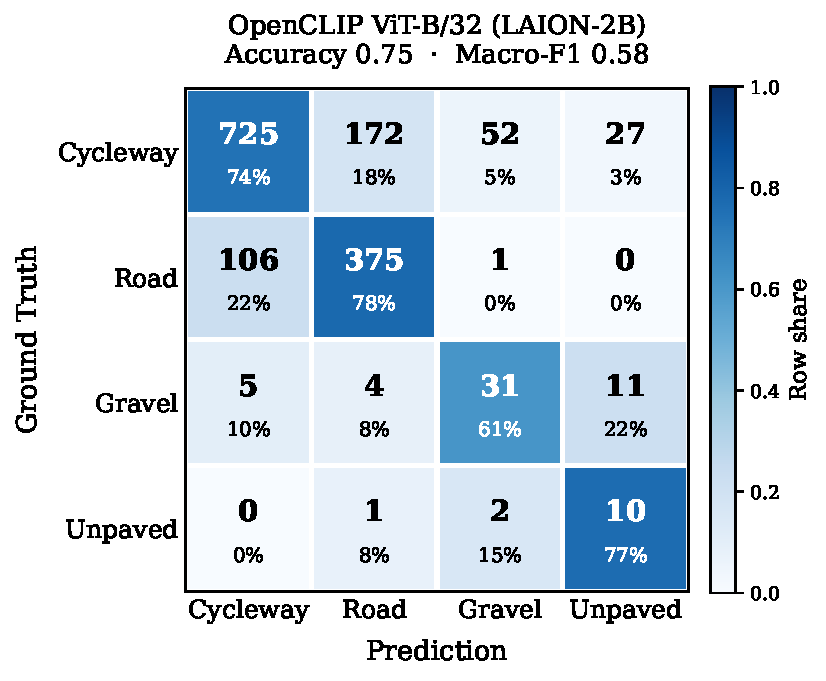
\includegraphics[width=0.91\columnwidth]{images/fig_confusion_best.pdf}
\caption{Row-normalized confusion matrix of the best model (OpenCLIP
ViT-B/32, LAION-2B) on the labeled test set. Each cell shows the count
and the row share; the diagonal is correct. Errors concentrate on the
Cycleway/Road pair and the rare Gravel/Unpaved classes.}
\label{fig:confusion}
\end{figure}

% =====================================================================
% PAGE 3 -- OBJECT DETECTION (not Bünyamin -- heading only)
% =====================================================================

\clearpage
\section{Object Detection}
% --- NOTE: This section will be written later. ---

% =====================================================================
% PAGE 4 -- ENVIRONMENT DETECTION (not Bünyamin -- heading only)
% =====================================================================

\clearpage
\section{Environment Detection: Zero-Shot vs.\ Fine-Tuned
Semantic Segmentation}

\emph{Environment detection} classifies each frame's surroundings and supplies the
environment sub-component -- the \emph{largest} score weight ($w_e = 0.45$,
Eq.~\eqref{eq:weights}). It is a \emph{multi-label whole-image} task: a frame may
show vegetation, water and a built-up scene at once, or none. We compare a
training-free vision--language model (CLIP~\cite{clip,urbanclip}) with a fine-tuned
semantic-segmentation transformer (SegFormer~\cite{segformer}) whose per-class
pixel-area fractions feed the sub-score directly (Eq.~\eqref{eq:env}).

\subsection{Task Type and Model Class}
\emph{Zero-shot CLIP} scores a per-class present-probability from prompt pairs,
needing no application-specific training. \emph{Fine-tuned SegFormer} predicts a
pixel mask whose class-area fractions are thresholded into presence -- richer than a
probability, and exactly what the beauty score consumes~\cite{greenery}. Both run at
edge speed.

\subsection{Environment Classes and Taxonomy}
Three classes are used: \textbf{Vegetation} (trees, grass, fields), \textbf{Water}
(river, lake or sea over ${\sim}2\%$ of the frame) and \textbf{City} (buildings or a
built-up street). The taxonomy was simplified from five to three: \emph{industry}
folded into \emph{City}, and the fuzzy \emph{forest}/\emph{open-field} pair -- the
weakest class -- merged into \emph{Vegetation} (the most impactful change,
Table~\ref{tab:seg-opt}, S9). SegFormer also learns an explicit \emph{``other''}
background class, so background is not forced into an environment class. Water is
intrinsically rare in street-level imagery, driving much of the optimization.

\subsection{Zero-Shot CLIP: Optimization}
Table~\ref{tab:clip-opt} lists the track. Two levers dominated: \emph{per-class
threshold calibration} on a leakage-free validation split ($+0.095$ macro-F1) and
\emph{prompt ensembling}~\cite{clip} over 6--8 templates per class ($+0.044$); model
capacity (ViT-L/14) did \emph{not} help. The water-inclusive final test then exposed
CLIP's water strength as a small-validation artifact (F1 $0.615$ val vs.\ $0.206$
test).

\begin{table}[!t]
\caption{CLIP zero-shot optimization (own-frames test). Final: ViT-B/32, prompt
ensembling, thresholds veg~$0.035$/water~$0.39$/city~$0.73$.}
\label{tab:clip-opt}
\centering
\scriptsize
\setlength{\tabcolsep}{2pt}
\renewcommand{\arraystretch}{1.0}
\begin{tabular}{@{}p{0.045\columnwidth}>{\raggedright\arraybackslash}p{0.5\columnwidth}>{\raggedright\arraybackslash}p{0.34\columnwidth}@{}}
\toprule
\textbf{\#} & \textbf{Optimization step} & \textbf{Effect / decision}\\
\midrule
C1 & Aligned prompt pairs, global threshold & baseline\\
C2 & Ride-disjoint val/test split & leakage-free tuning\\
C3 & Per-class threshold calibration & \textbf{+0.095}; top lever\\
C4 & Prompt ensembling, 6--8 templates~\cite{clip} & $+0.044$; adopted\\
C5 & Larger backbone ViT-L/14 & $-0.015$, 24$\times$ slower; rejected\\
C6 & 3-class taxonomy (veg.\ merge) & best config\\
C7 & Water-inclusive final test & water F1 $.62{\to}.21$: artifact\\
\bottomrule
\end{tabular}
\end{table}

\subsection{Fine-Tuned SegFormer: Optimization}
Table~\ref{tab:seg-opt} marks which steps were the fine-tuning itself (FT) versus
data or decision measures. The decisive gains were about \emph{data}: water is so
rare that a random Mapillary sample~\cite{mapillaryvistas} held almost none, so
class-balanced oversampling plus 258 ADE20K water scenes~\cite{ade20k} lifted water
IoU from $0$ to $0.70$. Swapping to an ADE20K-pretrained
base~\cite{ade20k,ftsegformer} (a water prior) and adding the ``other'' class raised
label-accuracy to $0.863$. An ablation (S10) values the fine-tuning itself at
$+0.027$ macro-F1, concentrated in \emph{City}.

\begin{table}[!t]
\caption{SegFormer optimization. \textbf{Type}: \emph{FT}$=$model (re)training,
\emph{data}$=$training data, \emph{eval}$=$decision. Final: B0 ADE20K base,
3~classes $+$ ``other'', thresholds veg~$0.25$/water~$10^{-4}$/city~$0.0056$.}
\label{tab:seg-opt}
\centering
\scriptsize
\setlength{\tabcolsep}{2pt}
\renewcommand{\arraystretch}{1.0}
\begin{tabular}{@{}p{0.05\columnwidth}>{\raggedright\arraybackslash}p{0.1\columnwidth}>{\raggedright\arraybackslash}p{0.42\columnwidth}>{\raggedright\arraybackslash}p{0.27\columnwidth}@{}}
\toprule
\textbf{\#} & \textbf{Type} & \textbf{Optimization step} & \textbf{Effect / decision}\\
\midrule
S1 & FT & Cityscapes-B0, random Mapillary~\cite{mapillaryvistas} & water F1 $0.00$ (baseline)\\
S2 & FT & Learning rate $6\!\times\!10^{-5}{\to}2\!\times\!10^{-4}$ & $+0.05$; water still $0$\\
S3--4 & data & Balanced $+$ water $\times2\text{--}6$ $+$ ADE water~\cite{ade20k} & water IoU $0{\to}0.70$: key fix\\
S5 & FT & Base swap $\to$ ADE20K (water prior)~\cite{ade20k} & water IoU $0.778$\\
S6 & data & Copy-paste water augmentation & water IoU $-0.11$; rejected\\
S8 & FT & Explicit ``other'' background class & label-acc $.65{\to}.86$\\
S9 & FT & 3-class taxonomy retrain & own-test macro $0.874$\\
S10 & eval & Fine-tuning ablation (no-FT) & FT worth $+0.027$\\
S11 & eval & Fine threshold grid ($\to 10^{-4}$) & \textbf{macro 0.704: wins}\\
\bottomrule
\end{tabular}
\end{table}

\subsection{Metrics and Protocol}
Both models are scored as multi-label classifiers on \textbf{macro-F1},
\textbf{label-accuracy} (mean per-(frame,\,class) correctness), \textbf{exact-match}
and \textbf{per-class F1} (mIoU during training). The headline set is
\textbf{1{,}210} cyclist-POV frames, ride-disjoint from all tuning
(983 / 40 / 307 veg/water/city positives); thresholds are fitted on a separate
validation split only.

\subsection{Results and Decision}
The fine-tuned SegFormer wins \emph{every} aggregate metric (macro-F1 $0.704$ vs.\
$0.649$; label-accuracy $0.911$ vs.\ $0.888$; exact-match $0.755$ vs.\ $0.691$) with
$40\times$ fewer parameters ($3.7$\,M vs.\ $151$\,M) at comparable latency
(Fig.~\ref{fig:env}); a per-class \emph{hybrid} was rejected ($\le 0.005$ gain).
\emph{Water is the shared limitation}: at best F1 $0.382$ the model is \emph{blind},
not miscalibrated ($68\%$ of true-water frames get almost no water pixels), because
in-domain water data is scarce -- so the clearest improvement is \emph{more
in-domain water frames in the fine-tuning set}, raising recall directly. SegFormer
is deployed, its area fractions feeding Eq.~\eqref{eq:env} directly.

\setlength{\intextsep}{4pt}%
\begin{figure}[H]
\centering
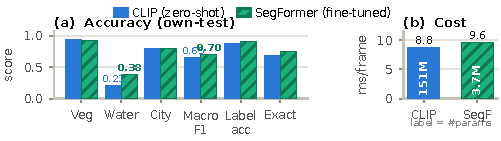
\includegraphics[width=\columnwidth]{images/fig_env_comparison}
\caption{Own-test (1{,}210 frames): \textbf{(a)}~per-class \& aggregate accuracy;
\textbf{(b)}~latency \& parameter count.}
\label{fig:env}
\end{figure}

% =====================================================================
% PAGE 5 -- BIKEABILITY SCORE (Bünyamin Aydemir)
% =====================================================================

\clearpage
\section{Computation of the Bikeability Score}

The bikeability score combines the three components (surface from
ground-detection, environment from environment-detection, and objects
from object-detection) into a single value in the interval $[0, 100]$.
Every detector emits a fixed-length \emph{vector}; each vector is first
mapped to a \emph{sub-score} in $[0,1]$, and the three sub-scores are
then combined by a weighted mean.

\subsection{Detector Outputs as Vectors}
The three detectors deliberately use different but fixed output
representations, each aligned element by element with a stored value
vector:
\begin{itemize}
\item \textbf{Ground}: a one-hot vector $\mathbf{g}\in\{0,1\}^{4}$ over
  the classes (Cycleway, Road, Gravel, Unpaved); exactly one entry is
  $1$.
\item \textbf{Environment}: a vector of area fractions
  $\mathbf{f}\in[0,1]^{3}$ over (vegetation, water, city).
\item \textbf{Object}: a vector of counts
  $\mathbf{n}\in\mathbb{Z}_{\ge 0}^{3}$ over (bicycle, car, traffic
  light).
\end{itemize}

\subsection{Overall Formula}
For each evaluated frame, the score $A$ results from the weighted mean
of the three sub-scores:
\begin{equation}
\label{eq:score}
A = 100 \cdot \Big( w_g \, S_{\text{ground}}
                  + w_e \, S_{\text{env}}
                  + w_o \, S_{\text{object}} \Big),
\end{equation}
with the weights
\begin{equation}
\label{eq:weights}
w_g = 0.20, \quad w_e = 0.45, \quad w_o = 0.35.
\end{equation}
The weights are heuristic and follow two considerations. Environment
and object exposure jointly capture how pleasant and how safe a stretch
feels, the factors a cyclist perceives most directly, and therefore
receive the larger share ($w_e + w_o = 0.80$). The surface receives the
smallest weight ($w_g = 0.20$): on typical routes it varies little, and
ground detection is also the least reliable component (macro-F1
$0.58$), so a smaller weight limits the influence of its errors. Since
all sub-scores lie in $[0,1]$ and the weights sum to $1$, the score is
bounded to $[0, 100]$. In practice the lower extreme $0$ is never
reached, as $S_{\text{ground}}\ge 0.1$ and
$S_{\text{object}}=\exp(-\max(\rho,0))>0$; the upper value $100$,
however, does occur whenever all three sub-scores equal $1$
simultaneously, e.g.\ on a paved cycleway ($S_{\text{ground}}=1$)
through vegetation or along water ($S_{\text{env}}=1$) with no
motorised traffic ($S_{\text{object}}=1$).

\subsection{Ground Sub-Score}
The ground sub-score is the inner product of the one-hot vector
$\mathbf{g}$ with the surface quality vector
$\mathbf{q}^{g}=(1.0,\,0.7,\,0.3,\,0.1)$ (Table~\ref{tab:quality}):
\begin{equation}
\label{eq:ground}
S_{\text{ground}} = \langle \mathbf{g},\, \mathbf{q}^{g}\rangle
                  = \sum_{k} g_k\, q^{g}_{k}.
\end{equation}
Because $\mathbf{g}$ is one-hot, this simply selects the quality of the
detected surface class.

\subsection{Environment Sub-Score}
The environment sub-score is the fraction-weighted mean of the
environment quality vector $\mathbf{q}^{e}=(1.0,\,1.0,\,0.4)$:
\begin{equation}
\label{eq:env}
S_{\text{env}} =
\begin{cases}
\dfrac{\langle \mathbf{f},\, \mathbf{q}^{e}\rangle}{\sum_{k} f_k},
  & \text{if } \sum_{k} f_k > 0,\\[2ex]
0.5, & \text{otherwise.}
\end{cases}
\end{equation}
The normalization by $\sum_k f_k$ keeps the sub-score in $[0,1]$ even
when the detected fractions do not cover the whole frame; a neutral
value of $0.5$ is used if no environment class is detected.

\subsection{Object Sub-Score}
The object sub-score maps the counts $\mathbf{n}$ through a
\emph{saturation function} using the penalty vector
$\boldsymbol{\lambda}=(-0.2,\,1.0,\,0.3)$:
\begin{equation}
\label{eq:object}
S_{\text{object}} = \exp\!\Big( -\max\big(\rho, 0\big) \Big),
\qquad
\rho = \langle \mathbf{n},\, \boldsymbol{\lambda}\rangle,
\end{equation}
where $\rho$ is evaluated independently per frame. A positive factor
for cars ($+1.0$) and traffic lights ($+0.3$) makes
$\rho$ positive and thus lowers the sub-score, whereas bicycles carry a
\emph{negative} factor ($-0.2$). The clamp $\max(\rho, 0)$ makes the
score asymmetric: a frame is never rewarded \emph{above} the neutral
value $1.0$, so bicycles do not inflate the score on their own; they
only \emph{offset} the penalty of nearby cars or traffic lights. This
encodes the intuition that good cycling conditions are the default and
only motorised traffic degrades them. The exponential form additionally
caps the influence of outliers, so a single crowded frame cannot
dominate the overall score.

\begin{table}[H]
\caption{Class value vectors for the three sub-scores: surface quality
$\mathbf{q}^{g}$, environment quality $\mathbf{q}^{e}$, and object
weight $\boldsymbol{\lambda}$ (heuristic; a negative value acts as a
bonus).}
\label{tab:quality}
\centering
\begin{tabular}{@{}llc@{}}
\toprule
\textbf{Component} & \textbf{Class} & \textbf{Value}\\
\midrule
\multirow{4}{*}{Ground $\mathbf{q}^{g}$}
  & Cycleway & $1.0$\\
  & Road     & $0.7$\\
  & Gravel   & $0.3$\\
  & Unpaved  & $0.1$\\
\midrule
\multirow{3}{*}{Environment $\mathbf{q}^{e}$}
  & Vegetation & $1.0$\\
  & Water      & $1.0$\\
  & City       & $0.4$\\
\midrule
\multirow{3}{*}{Object weight $\boldsymbol{\lambda}$}
  & Bicycle       & $-0.2$\\
  & Car           & $+1.0$\\
  & Traffic light & $+0.3$\\
\bottomrule
\end{tabular}
\end{table}

\subsection{GPX Mapping and Visualization}
Because the camera clock is unreliable, the frames are aligned to the
GPS track by a single \emph{manual sync point} (by default: recording
start $=$ GPX track start). Each frame is then matched to its nearest
GPX track point in time (a nearest-neighbor join within a $3$\,s
tolerance: large enough to bridge gaps in the roughly $1$\,Hz GPS
log, yet below the $5$\,s frame spacing so that each frame maps to a
distinct track point), which assigns a latitude/longitude to every
score. The \emph{average} bikeability score of the route is the mean
$\bar{A} = \frac{1}{M}\sum_{i=1}^{M} A_i$ over all $M$ evaluated frames.
Finally, the route is drawn as a sequence of short segments, each
colored by the local score on a red--orange--yellow--green scale
(Fig.~\ref{fig:route}). For the example ride shown, the mean score is
$\bar{A}\approx 85.7/100$: the track is predominantly green (good
cycling conditions) with a few yellow/orange sections.

\begin{figure}[H]
\centering
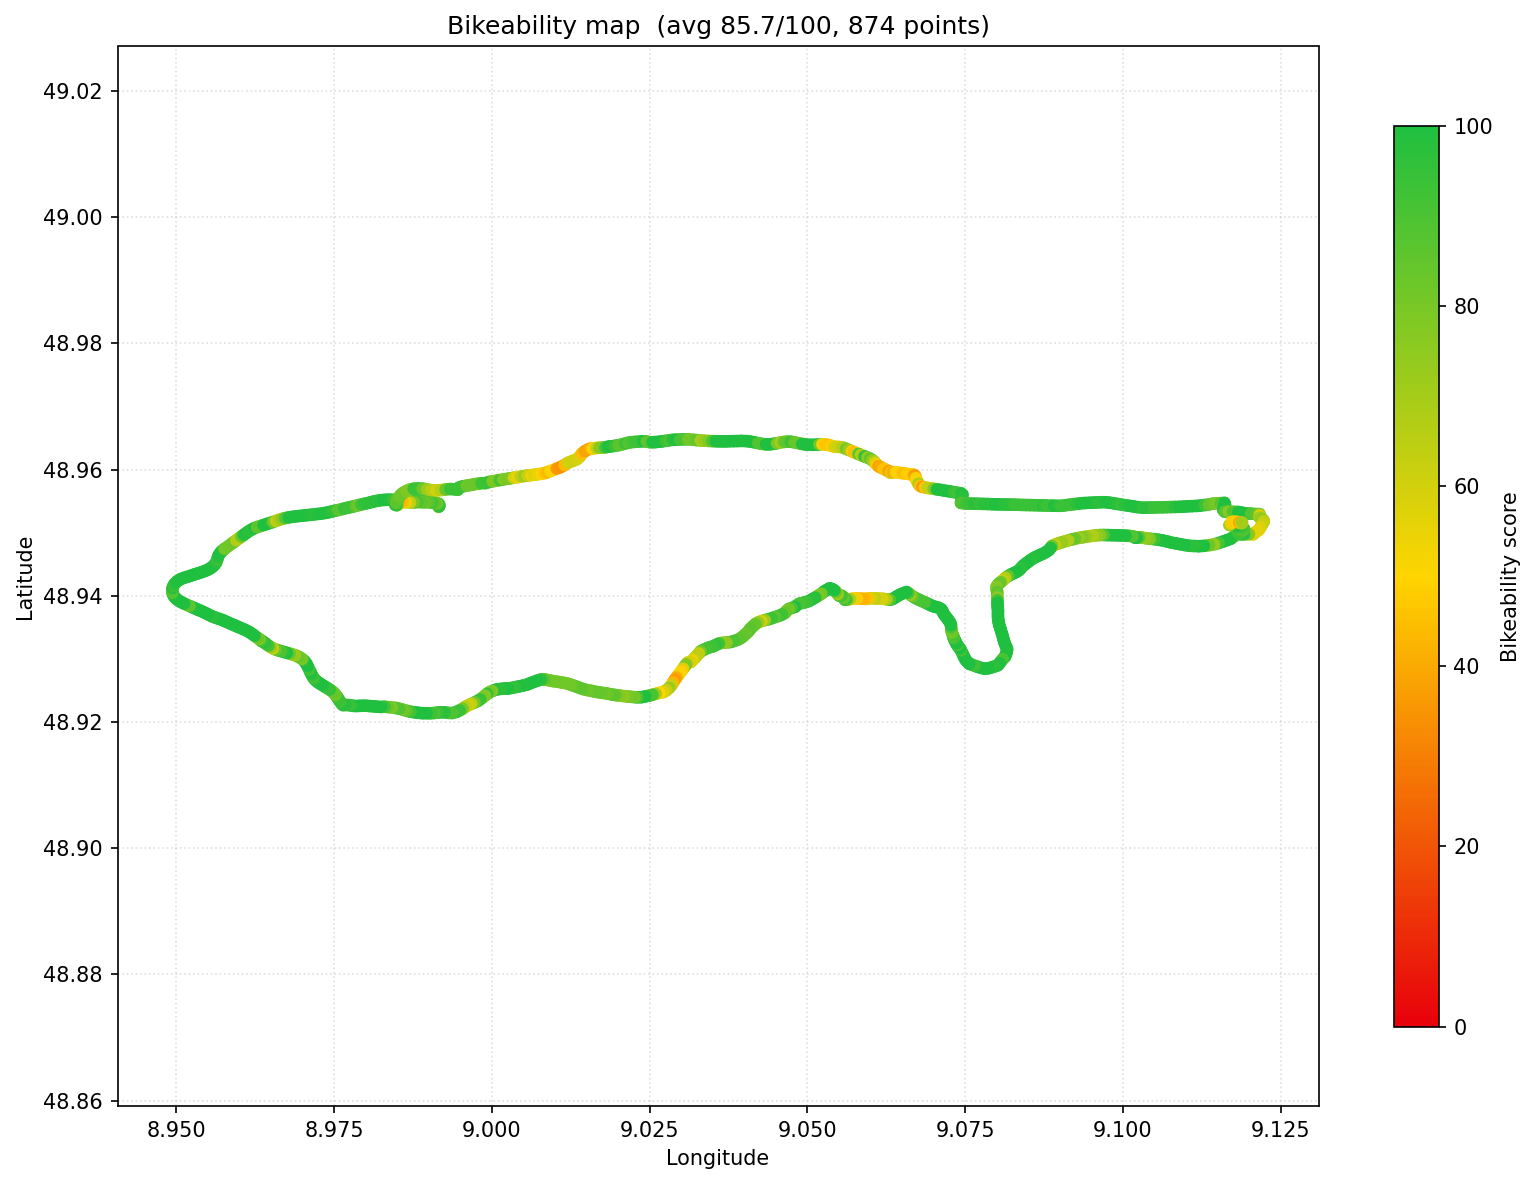
\includegraphics[width=\columnwidth]{images/bikeability_map.png}
\caption{Bikeability score colored along the GPX route (red $=$ low,
green $=$ high). Per-frame scores are matched to the nearest GPS track
point via a manual sync point; the example ride has a mean score of
$\bar{A}\approx 85.7/100$.}
\label{fig:route}
\end{figure}

% =====================================================================
% DISCUSSION (to be written later, heading only)
% =====================================================================

\section{Discussion}
% --- NOTE: This section will be written later. ---

% =====================================================================
% CONCLUSION (to be written later, heading only)
% =====================================================================

\section{Conclusion}
% --- NOTE: This section will be written later. ---

% =====================================================================
% Bibliography
% =====================================================================

\bibliographystyle{IEEEtran}
\bibliography{references}

\end{document}
